\subsection{Caso d'uso UC6: Esportazione della presentazione}
	\begin{figure}[h]
		\centering
		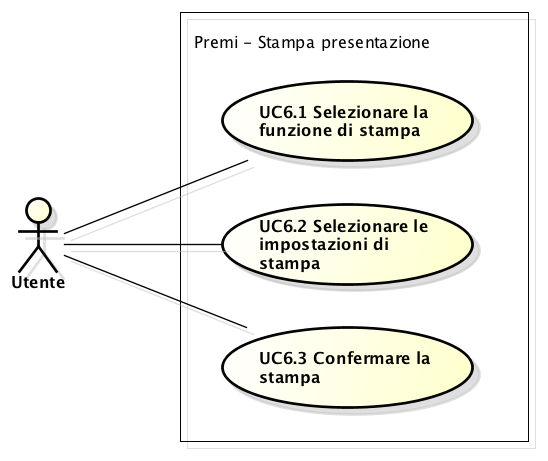
\includegraphics[scale=0.45] {img/UC6.png}
		\caption{UC6 - Esportazione della presentazione}
	\end{figure}

	\begin{itemize}
		\item \textbf{Attori:} Utente;
		\item \textbf{Scopo e descrizione:} L'utente ha creato una presentazione di slide e vuole esportarla nel proprio computer;
		\item \textbf{Precondizione:} Il sistema è in attesa che l'utente selezioni la funzione esporta;
		\item \textbf{Flusso degli eventi:}
		\begin{enumerate}
			\item L'utente seleziona dal menù la funzione esporta [UC6.1];
			\item L'utente seleziona il formato in cui esportare la presentazione [UC6.2];
			\item L'utente seleziona la cartella nella quale esportare la presentazione [UC6.3];
			\item L'utente seleziona il percorso di destinazione [UC6.5];
			\item L'utente conferma l'esportazione [UC6.4];
		\end{enumerate}
		\item \textbf{Postcondizione:} Il sistema ha esportato la presentazione.
	\end{itemize}


\subsection{Caso d'uso UC6.1: Selezionare funzione esporta}
	\begin{itemize}
		\item \textbf{Attori:} Utente;
		\item \textbf{Scopo e descrizione:} L'utente seleziona dall'apposito menù la funzione di esportazione per esportare la presentazione;
		\item \textbf{Precondizione:} Il sistema è in attesa che l'utente selezioni la funzione esporta;
		\item \textbf{Postcondizione:} Il sistema apre la finestra di dialogo per l'esportazione.
	\end{itemize}


\subsection{Caso d'uso UC6.2: Selezionare il formato di esportazione}
	\begin{itemize}
		\item \textbf{Attori:} Utente;
		\item \textbf{Scopo e descrizione:} L'utente seleziona il formato in cui esportare la presentazione;
		\item \textbf{Precondizione:} Il sistema è in attesa che l'utente selezioni il formato dall'apposita finestra di dialogo;
		\item \textbf{Postcondizione:} Il sistema registra la scelta fatta dall'utente.
	\end{itemize}


\subsection{Caso d'uso UC6.3: Selezionare la destinazione di esportazione}
	\begin{itemize}
		\item \textbf{Attori:} Utente;
		\item \textbf{Scopo e descrizione:} L'utente deve scegliere la destinazione in cui salvare la presentazione esportata.
		\item \textbf{Precondizione:} Il sistema è in attesa che l'utente selezioni il percorso dall'apposita finestra di dialogo;
		\item \textbf{Postcondizione:} Il sistema registra la destinazione desiderata.
	\end{itemize}


\subsection{Caso d'uso UC6.4: Confermare l'esportazione}
	\begin{itemize}
		\item \textbf{Attori:} Utente;
		\item \textbf{Scopo e descrizione:} L'utente conferma l'esportazione nel formato e nella destinazione desiderati;
		\item \textbf{Precondizione:} Il sistema è in attesa che l'utente confermi l'esportazione;
		\item \textbf{Postcondizione:} Il sistema ha esportato la presentazione.
	\end{itemize}


\subsection{Caso d'uso UC6.5: Selezionare il percorso}
	\begin{figure}[h]
		\centering
		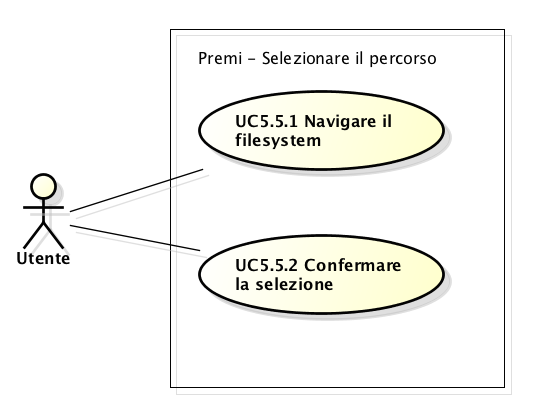
\includegraphics[scale=0.45] {img/UC6.5.png}
		\caption{UC6.5 - Selezionare il percorso}
	\end{figure}
	\begin{itemize}
		\item \textbf{Attori:} Utente;
		\item \textbf{Scopo e descrizione:} L'utente deve scegliere il percorso. Naviga il \gls{filesystem}, lo seleziona ne e conferma la scelta;
		\item \textbf{Precondizione:} Il sistema è in attesa che l'utente navighi il \gls{filesystem} e confermi il percorso scelto;
		\item \textbf{Flusso degli eventi:}
		\begin{enumerate}
			\item L'utente naviga il \gls{filesystem} alla ricerca della posizione desiderata [UC6.5.1];
			\item L'utente conferma la posizione selezionata [UC6.5.2].
		\end{enumerate}
		\item \textbf{Postcondizione:} Il sistema registra il percorso desiderato.
	\end{itemize}

	\subsection{Caso d'uso UC6.5.1: Navigare il filesystem}
	\begin{itemize}
		\item \textbf{Attori:} Utente;
		\item \textbf{Scopo e descrizione:} L'utente naviga il \gls{filesystem} per selezionare la cartella dentro la quale vuole esportare la presentazione;
		\item \textbf{Precondizione:} Il sistema è in attesa che l'utente selezioni una cartella;
		\item \textbf{Postcondizione:} Il sistema ha aggiornato il percorso.
	\end{itemize}

	\subsection{Caso d'uso UC6.5.2: Confermare selezione}
	\begin{itemize}
		\item \textbf{Attori:} Utente;
		\item \textbf{Scopo e descrizione:} L'utente conferma che il percorso selezionato è quello corretto;
		\item \textbf{Precondizione:} Il sistema ha selezionato il percorso indicato dall'utente;
		\item \textbf{Postcondizione:} Il sistema ha registrato il percorso scelto.
	\end{itemize}
